\documentclass[11pt,letterpaper]{article}                  % Define document class

%! Mandatory packages
\usepackage[utf8]{inputenc}                                %! Character encoding
\usepackage[T1]{fontenc}                                   %! Font encoding
\usepackage[english]{babel}                                %! Language setting

% Set path
\newcommand{\path}{Preamble}

% Text packages
% Text packages
\usepackage[margin=1in]{geometry}                          % Margin size
\usepackage{enumerate}                                     % Custom enumeration lists
\usepackage{footmisc}                                      % Stable footnotes in headings
\usepackage{natbib}                                        % Bibliography
\usepackage{hyperref}                                      % Hyperreferences
    \hypersetup{
      colorlinks,
      citecolor=black,
      filecolor=black,
      linkcolor=black,
      urlcolor=blue
    }
\usepackage[]{authblk}                                     % Affiliation in maketitle
    \renewcommand\Affilfont{\small}                        % Small font size for affiliation
\usepackage{multicol}                                      % Multiple columns in text
\usepackage[nointegrals]{wasysym}                          % WASY2 symbols for contradiction \lightning
\usepackage{lmodern}                                       % Latin Modern font for correct T1 font encoding (no pixelated output)
\usepackage{algorithm}                                     % Pseudocode packages
\usepackage{algpseudocode}
\setlength\parindent{0pt}                                  % No indentation for the whole document

% Figure/table packages
% Figure and table packages
\usepackage{float}                                         % Figure floats
\usepackage[position=top]{subfig}                          % Subfigures
\usepackage{multirow}                                      % Merged rows in tables
\usepackage{dcolumn}                                       % Custom table delimiters
\usepackage[labelfont=bf, font=normalsize]{caption}        % Bold captions
    \captionsetup{format=hang}

% Math packages
% Math packages
\usepackage{amsmath}                                       % AMS math package
\usepackage{amssymb}                                       % Math symbols
\usepackage{amsthm}                                        % Custom theorem environments
%\usepackage{units}                                         % Numerical fractions
\usepackage{centernot}                                     % Logical negation in the middle of characters; e.g. not iff

% Custom theorems
% E.g. \newtheorem{command}[counter]{Display name}
\newtheorem{theorem}{Theorem}[]
\newtheorem{acknowledgement}[theorem]{Acknowledgment}
\newtheorem{axiom}[theorem]{Axiom}
\newtheorem{case}[theorem]{Case}
\newtheorem{claim}[theorem]{Claim}
\newtheorem{conclusion}[theorem]{Conclusion}
\newtheorem{condition}[theorem]{Condition}
\newtheorem{conjecture}[theorem]{Conjecture}
\newtheorem{corollary}[theorem]{Corollary}
\newtheorem{criterion}[theorem]{Criterion}
\newtheorem{exercise}[theorem]{Exercise}
\newtheorem{lemma}[theorem]{Lemma}
\newtheorem{notation}[theorem]{Notation}
\theoremstyle{definition}
\newtheorem*{definition}{Definition}
\newtheorem*{altdef}{Alternative definition}
\newtheorem{problem}[theorem]{Problem}
\newtheorem{assumption}[theorem]{Assumption}
\newtheorem{proposition}[theorem]{Proposition}
\theoremstyle{remark}
\newtheorem{example}[theorem]{Example}
\newtheorem{remark}[theorem]{Remark}
\newtheorem{solution}[theorem]{Solution}
\newtheorem{summary}[theorem]{Summary}

\renewcommand{\qedsymbol}{$\blacksquare$}                  % QED

% Mathematical operators
\DeclareMathOperator{\E}{E}                                % Expected value
\DeclareMathOperator{\var}{var}                            % Variance
\DeclareMathOperator{\cov}{cov}                            % Covariance
\DeclareMathOperator{\corr}{corr}                          % Correlation
\DeclareMathOperator{\avar}{avar}                          % Asymptotic variance
\DeclareMathOperator{\plim}{plim}                          % Probability limit
\DeclareMathOperator{\lag}{lag}                            % Lag operator
\DeclareMathOperator{\rank}{rank}                          % Rank
\DeclareMathOperator{\I}{I}                                % Identity matrix

\providecommand{\abs}[1]{\left\lvert#1\right\rvert}        % Absolute value
\providecommand{\norm}[1]{\left\lVert#1\right\rVert}       % Norm
\providecommand{\ip}[1]{\left\langle#1\right\rangle}       % Inner product
\providecommand{\csp}{\overline{\mathrm{sp}}}              % Closed span
\providecommand{\pto}{\overset{p}{\to}}                    % Convergence in probability
\providecommand{\dto}{\overset{d}{\to}}                    % Convergence in distribution

% Graphics packages
% Graphics packages
\usepackage{tikz}                                          % TikZ drawings
\usepackage{pgfplots}                                      % PGFPlots plots
    \pgfplotsset{                                          % PGFPlots options
        cartesian/.style={                                 % Declaring Cartesian plane style
            % Axis alignment
            axis x line=middle,
            axis y line=middle,
            % Axis labels alignment
            every axis x label/.style={at={(current axis.right of origin)},anchor=north west},
            every axis y label/.style={at={(current axis.above origin)},anchor=north east},
            % Legend alignment
            every axis legend/.append style={legend pos=outer north east}
        },
        % Version declaration for compatibility
        compat=1.11
    }
\usetikzlibrary{calc}
    % Node setup for extensive form games
    \tikzset{
        % Two node styles for game trees: solid and hollow
        solid node/.style={circle,draw,inner sep=1.5,fill=black},
        hollow node/.style={circle,draw,inner sep=1.5},
        % Solution nodes
        solidsol node/.style={blue,circle,draw,inner sep=1.5,fill=blue},
        hollowsol node/.style={blue,circle,draw,inner sep=1.5}
    }


% Title
\title{Problem Set 1 \\ \medskip \Large{Econometrics III}}
\author{\Large Jackson Bunting, Attila Gyetvai, Peter Horvath, Leonardo Salim Saker Chaves\footnote{Department of Economics, Duke University}}
\date{\today}

%%%%%%%%%%%%%%%%%%%%%%%%%%%%%%%%%

\begin{document}

\maketitle

\begin{problem}

\end{problem}

\bigskip

\begin{problem}

\end{problem}

\bigskip

\begin{problem}
Let $\{X_i\}_{i \in \mathbb{N}}$ be a sequence of random variables with mean $\mu$. Suppose that $Cov(X_t,X_s)=0 \forall t\neq s$ and $Var(X_t) \leq Kt^{1/2}$ for some constant $K>0$. Show that $\bar{X_t} \overset{\mathbb{P}}{\rightarrow} \mu$.\\

\textbf{Solution:} Consider any $\epsilon>0$. Using Markov inequality we get
\begin{align*}
P(|\bar{X_t} - \mu| > \epsilon) &\leq \frac{\mathbb{E}( |\bar{X_t} - \mu|^2)}{\epsilon^2} = \frac{V(\bar{X_t})}{\epsilon^2} \\
&\leq \frac{\sum_{t=1}^T V(X_t)}{T^2 \epsilon^2} = \frac{K \sum_{t=1}^T t^{1/2}}{T^2 \epsilon^2} \\
&\leq \frac{K T^{3/2}}{T^2 \epsilon^2} \overset{t \to \infty}{\longrightarrow} 0
\end{align*}

Then $\bar{X_t} - \mu \overset{\mathbb{P}}{\rightarrow} 0$ which is equivalent to what we wanted to show.
\end{problem}

\bigskip

\begin{problem}

\end{problem}

\bigskip

\begin{problem}
Suppose that $\sup_{t \in \mathcal{T}} \mathbb{E}(|X_t|^{1+\delta}) < \infty$ for some $\delta >0$. Then $\{X_t : t \in \mathcal{T}\}$ is uniformly integrable. (Hint: Markov's inequality) \\

\textbf{Solution:} Notice that $\sup_{t \in \mathcal{T}} \mathbb{E}(|X_t|I_{[|X_t|>M]}) \leq \sup_{t \in \mathcal{T}} \mathbb{E}(|X_t|) \sup_{t \in \mathcal{T}}P(X_t >M)$.

From Markov inequality we have
\begin{align*}
P(|X_t|>M)&\leq \frac{\mathbb{E}(|X_t|^{1+\delta})}{M^{1+\delta}} \\
&< \frac{\eta}{M^2} \overset{M \to \infty}{\longrightarrow} 0
\end{align*}
Moreover, assuming $\sup_{t \in \mathcal{T}} \mathbb{E}(|X_t|^{1+\delta}) < \infty$ implies that $\sup_{t \in \mathcal{T}} \mathbb{E}(|X_t|)<\infty$.

All of it implies that $\lim_{M \to \infty} \sup_{t \in \mathcal{T}} \mathbb{E}(|X_t| I_{[X_t| > M]}) \leq 0$. Since $|X_t| I_{[X_t| > M]}\geq 0$, we get the uniform integrability of $\{X_t : t \in \mathcal{T}\}$.
\end{problem}

\bigskip

\begin{problem}

\end{problem}

\bigskip

\begin{problem}

\end{problem}

\bigskip

\begin{problem}

\end{problem}

\bigskip

\begin{problem}

\end{problem}

\bigskip

\begin{problem}
Let $a_n = o_p(1)$.
Interpret and prove that $O_p(a_n) = o_p(1)$. \\

\textbf{Solution:} If I divide $X_n$ by $a_n = o_p(1)$, it has to be the case that $X_n  = o_p(1)$.
The proof is as it follows:
\begin{align*}
  X_n &= O_p (a_n) \iff \frac{X_n}{a_n} = O_p(1); \\
  X_n &= \frac{X_n}{a_n} \, a_n = O_p(1) \, o_p(1) = o_p(1)
\end{align*}
The first line is just the definition of $O_p(a_n)$.
The second line comes from the $o_p$--$O_p$ identities in the notes.
\end{problem}

\bigskip

\begin{problem}
Interpret and prove that $e^{o_p(1)} -1 = o_p(1)$ and $(O_p(1))^{\sqrt{2}} = O_p(1)$. \\

\textbf{Solution:} If you pick a r.v. $X = o_p(1)$, then a continuous transformation will also be $o_p(1)$. The proof is a straightforward consequence of CMT.

For the second claim, the interpretation is that you preserve $O_p(1)$ property when you take a continuous function of this r.v.. To prove, let $X_n = O_p(1)$. By definition, $\exists M>0 ; \sup_{n \in \mathbb{N}} P(|X_n|>M)<\epsilon)$. Notice that $\{\omega \in \Omega : |X_n(\omega)|>M\} = \{\omega \in \Omega : |X_n(\omega)|^{\sqrt{2}}>M^{\sqrt{2}}\}$ because it is a monotonic transformation. Thus, $\exists \eta = M^{\sqrt{2}}>0 ; \sup_{n \in \mathbb{N}} P(|X_n^{\sqrt{2}}|>\eta)<\epsilon)$.
\end{problem}

\bigskip

\begin{problem}
Let $f(x) = \exp (x^2)$.
Let $(X_i)_{1 \leq i \leq n}$ be iid $N(\mu,1)$ variables.
Simulate such a sequence with $n = 100$ and $\mu = 0.3$.
Compute $f (\bar{X})$ where $\bar{X} = \frac{1}{n} \sum_{i=1}^n X_i$.
Repeat this for 2000 times. Plot the distribution of $f (\bar{X})$ in the simulation.
What is the asymptotic distribution of $f (\bar{X})$?
Is the asymptotic distribution a good approximation to the empirical distribution?
Repeat for $\mu =$ 0, 0.1, 0.2, 0.3, 0.4, 0.5.
Discuss the results. \\

\textbf{Solution:}
We plot the simulated empirical distributions below.
For $\mu = 0$, the distribution is skewed to the right, resembling the $\chi^2$-distribution.
As $\mu$ increases (especially after $\mu \geq 0.4$), the distribution gets closer and closer to normal.

\begin{figure}[H]
  \centering
  \caption{Simulated empirical distributions}
  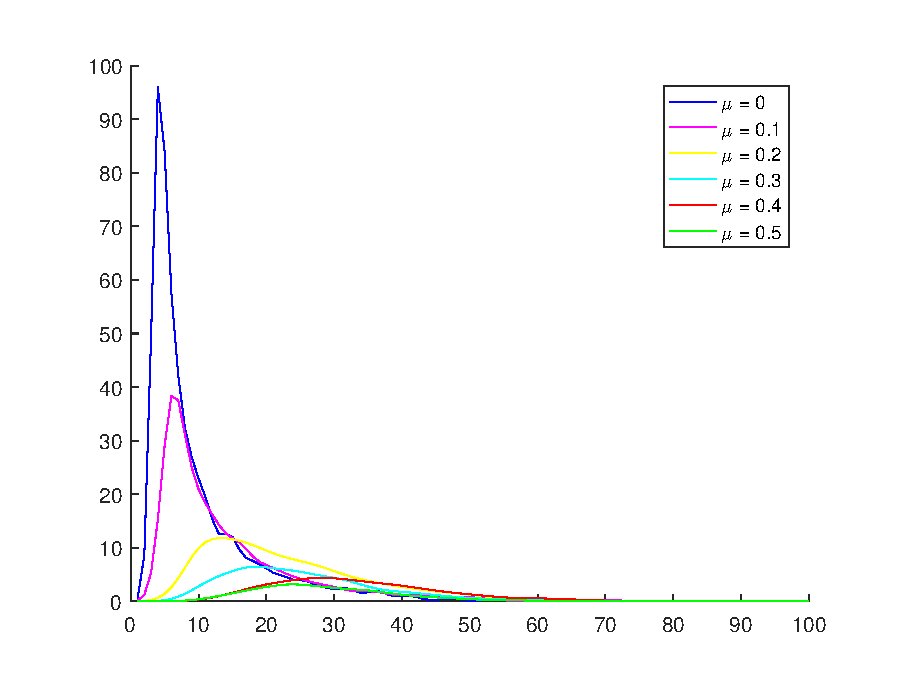
\includegraphics[scale=0.6]{prob12.eps}
\end{figure}
\end{problem}

\bigskip

\begin{problem}

\end{problem}


\end{document}